\textbf{Input data and beam properties.} For $L=0.445\,\mathrm m$, $h=3.00\,\mathrm{mm}$, $b=37.0\,\mathrm{mm}$, $E=200\,\mathrm{GPa}$, and $\rho=7850\,\mathrm{kg/m^3}$, the rectangular cross section gives
\[
A=bh=111\,\mathrm{mm^2},\quad m=\rho A=0.871\,\mathrm{kg/m},\quad
I=\frac{bh^3}{12}=8.33\times10^{-11}\,\mathrm{m^4},
\]
\[
EI=16.7\,\mathrm{N\,m^2},\qquad a=\left(\frac{EI}{m}\right)^{1/4}=2.09\,\mathrm{m/\sqrt{s}}.
\]
For mode 1, the first root $z_1=4.73004$ gives $\gamma_1=4.73004/0.445=10.63\,\mathrm{rad/m}$, $\omega_1=a^2\gamma_1^2=493.9\,\mathrm{rad/s}$, and $f_1=78.60\,\mathrm{Hz}$. The remaining frequencies follow the same substitution using their respective roots.

The free-end conditions $W''=W'''=0$ at both ends yield $\cos z\cosh z-1=0$. I solve the equivalent equation $\cos z-\operatorname{sech}z=0$ for its first five positive flexural roots. The free beam also has two zero-frequency rigid-body modes, translation and rotation. The following table gives the flexible modes using $\gamma_j=z_j/L$, $\omega_j=a^2\gamma_j^2$, and $f_j=\omega_j/(2\pi)$.
\begin{center}
\begin{tabular}{rrrrrr}\toprule
$j$ & $z_j$ & $\gamma_j$ (rad/m) & $\omega_j$ (rad/s) & $f_j$ (Hz) & $\beta_j$\\ \midrule
1 & 4.73004 & 10.63 & 493.9 & 78.60 & 0.982502\\
2 & 7.85320 & 17.65 & 1361 & 216.7 & 1.000777\\
3 & 10.9956 & 24.71 & 2669 & 424.8 & 0.999966\\
4 & 14.1372 & 31.77 & 4412 & 702.2 & 1.000001\\
5 & 17.2788 & 38.83 & 6590 & 1049 & 1.000000\\ \bottomrule
\end{tabular}
\end{center}

\textbf{Modes and orthonormality.} Following the course notes, PDF pages 185--191, the coefficient and flexible mode are
\[
\beta_j=\frac{\cosh z_j-\cos z_j}{\sinh z_j-\sin z_j},\quad
W_j(x)=\cosh\gamma_jx+\cos\gamma_jx-\beta_j(\sinh\gamma_jx+\sin\gamma_jx).
\]
To compare modes on a common scale, define $\phi_j=W_j/\sqrt{L^{-1}\int_0^L W_j^2\,dx}$. Then $L^{-1}\int_0^L\phi_j\phi_k\,dx=\delta_{jk}$. Each mode is rescaled so that $L^{-1}\int_0^LW_j^2\,dx=1$. The five individual modes and their overlay appear below. Trapezoidal integration at 1001 equally spaced points gives diagonal entries of one and a maximum off-diagonal magnitude of $1.88\times10^{-5}$ in $L^{-1}\int_0^LW_jW_k\,dx$. Symmetric and antisymmetric modes alternate, and frequency rises with mode number.

\begin{figure}[H]\centering
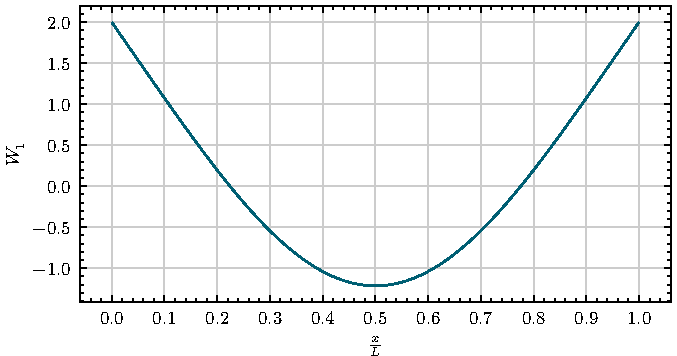
\includegraphics[width=0.46\linewidth]{figures/generated/solutions/C3_mode1.pdf}
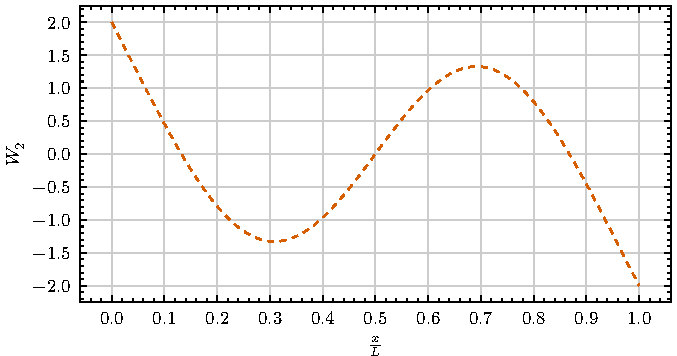
\includegraphics[width=0.46\linewidth]{figures/generated/solutions/C3_mode2.pdf}
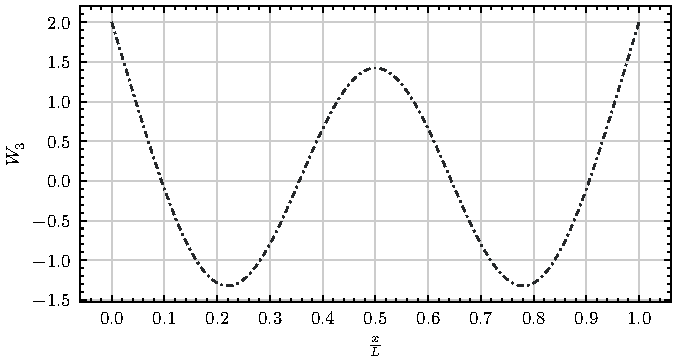
\includegraphics[width=0.46\linewidth]{figures/generated/solutions/C3_mode3.pdf}
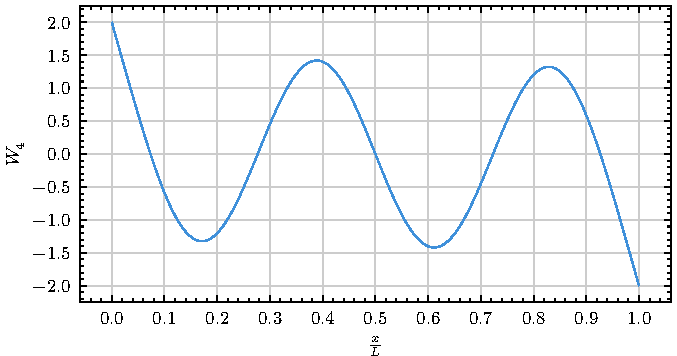
\includegraphics[width=0.46\linewidth]{figures/generated/solutions/C3_mode4.pdf}
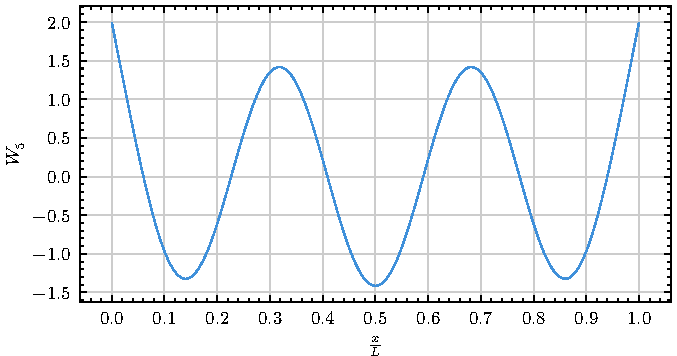
\includegraphics[width=0.46\linewidth]{figures/generated/solutions/C3_mode5.pdf}
\caption{First five flexible free-free beam modes.}
\end{figure}
\begin{figure}[H]\centering
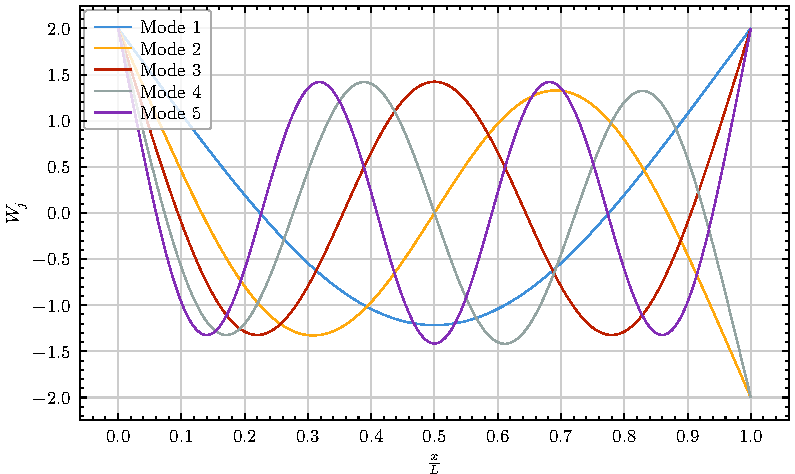
\includegraphics[width=0.8\linewidth]{figures/generated/solutions/C3.pdf}
\caption{Overlay of the first five flexible free-free beam modes.}
\end{figure}
\lstinputlisting[style=hwmatlab,caption={Free-free beam modal calculation.}]{matlab/C3.m}
